\documentclass[11pt,a4paper]{article}

\usepackage[utf8]{inputenc}
\usepackage[italian]{babel}
\usepackage{amsmath,amssymb} 
\usepackage{graphicx}        
\usepackage{booktabs}        
\usepackage{hyperref}     
\usepackage{geometry}
\usepackage{float}
\usepackage{tabularx}
\usepackage{placeins}
\usepackage{url} 

\geometry{a4paper, top=3cm, bottom=3cm, left=2.5cm, right=2.5cm}

\hypersetup{
    colorlinks=true,
    linkcolor=blue,
    filecolor=magenta,      
    urlcolor=cyan,
    pdftitle={Relazione Progetto Data Science},
}



\usepackage{graphicx} 

\title{Analisi predittiva dell'abbandono aziendale: il Fenomeno dell'Employee Attrition}
\author{Amoroso G., Guarnieri F. e Kovacs E.E.}
\date{Anno accademico 2025/2026}

\begin{document}

\maketitle

\section{Introduzione}
Nel contesto attuale delle organizzazioni, la gestione delle risorse umane rappresenta un fattore cruciale per il successo aziendale. In particolare, il fenomeno dell’attrition, ovvero l’abbandono dei dipendenti, può avere impatti significativi sia in termini economici che organizzativi, comportando costi legati alla sostituzione del personale e alla perdita di competenze.

Lo scopo di questo progetto è analizzare il dataset \texttt{Employee\_Attrition} al fine di comprendere quali fattori influenzano la probabilità che un dipendente lasci l'azienda e costruire modelli computazionali in grado di prevedere tale evento. Il dataset contiene informazioni relative a caratteristiche demografiche, professionali e di soddisfazione dei dipendenti, tra cui l'età, il ruolo lavorativo, il reddito mensile, il livello di soddisfazione e l'equilibrio tra vita lavorativa e personale (\textit{work-life balance}).

Attraverso un approccio rigoroso di data science, il progetto è stato sviluppato seguendo un ciclo di vita strutturato, volto a garantire l'organizzabilità, la tracciabilità e la riproducibilità dell'analisi attraverso le seguenti sei macro-fasi operative:
\begin{enumerate}
    \item \textbf{Setup del progetto:} Configurazione dell'ambiente di lavoro e del repository remoto sulla piattaforma di versionamento GitHub per il tracciamento cooperativo del codice.
    \item \textbf{Descrizione e comprensione del dataset:} Analisi preliminare della struttura dei dati, controllo della qualità delle informazioni e formulazione delle ipotesi di ricerca iniziali.
    \item \textbf{Analisi esplorativa e visualizzazione (EDA):} Studio approfondito delle relazioni tra le \textit{feature} e la variabile target, identificando sfide intrinseche del dominio come il forte sbilanciamento delle classi (\textit{class imbalance}).
    \item \textbf{Modellazione:} Preprocessing dei dati (trattamento dei dati mancanti, codifica delle variabili categoriche e \textit{train/test split}) e addestramento di diversi algoritmi di machine learning per la classificazione.
    \item \textbf{Valutazione e interpretazione dei risultati:} Analisi critica delle performance dei modelli tramite metriche statistiche standardizzate (accuratezza, precisione, recall, f1-score e matrici di confusione).
    \item \textbf{Report scientifico:} Sintesi formale e interpretazione scientifica delle evidenze riscontrate, redatta in ambiente \LaTeX{}.
\end{enumerate}

L'obiettivo finale è quindi duplice: da un lato fornire uno strumento predittivo accurato per identificare tempestivamente i dipendenti a rischio di abbandono, e dall'altro ottenere \textit{insight} significativi e statisticamente giustificati che possano supportare decisioni strategiche e proattive in ambito HR 

Il presente report è strutturato in modo da riflettere fedelmente questo percorso metodologico e si organizza nelle sezioni: Introduzione, Dataset, Analisi Esplorativa dei dati (EDA), Modellazione, Risultati e discussione e Conclusioni.

Tutto il codice sorgente, i notebook computazionali eseguiti e i file di configurazione associati a questo studio sono consultabili presso il repository GitHub del progetto: \\
\url{https://github.com/evelinenikokovacs/Employee_Attrition}

\section{Dataset}
\subsection{Descrizione e struttura dei dati}
Il dataset utilizzato in questo studio è denominato \texttt{Employee\_Attrition} ed è composto da un campione di $1470$ osservazioni (dipendenti) e $35$ variabili complessive. L'obiettivo primario dell'analisi consiste nel modellare una funzione predittiva in grado di mappare le caratteristiche del dipendente verso la variabile target $Y$, definita come:

\begin{equation}
Y = \text{\texttt{Attrition}} = 
\begin{cases} 
1 & \text{se il dipendente ha lasciato l'azienda (\textit{Yes})} \\
0 & \text{altrimenti (\textit{No})}
\end{cases}
\end{equation}

Il dataset presenta una struttura informativa eterogenea, che consente di suddividere le $34$ feature predittive ($X_i$) in tre macro-categorie tassonomiche:
\begin{itemize}
    \item \textbf{Caratteristiche Demografiche e Personali:} \texttt{Age} (età quantitativa continua), \texttt{Gender} (nominale binaria), \texttt{MaritalStatus} (nominale politomica: \textit{Single, Married, Divorced}) e \texttt{DistanceFromHome} (distanza casa-lavoro in km).
    \item \textbf{Metriche Professionali ed Economiche:} \texttt{JobRole} (ruolo occupato), \texttt{MonthlyIncome} (reddito mensile lordo), \texttt{YearsAtCompany} (anzianità aziendale), \texttt{TotalWorkingYears} (anni complessivi di carriera) e \texttt{OverTime} (presenza di lavoro straordinario, variabile binaria \textit{Yes/No}).
    \item \textbf{Valutazioni Psicometriche e di Performance:} Variabili qualitative discrete misurate su scala Likert ordinale a 4 livelli (da $1$ a $4$), volte a quantificare la percezione soggettiva dell'ambiente lavorativo.
\end{itemize}

Per garantire la massima chiarezza interpretativa, la mappatura dei codici numerici per le principali scale ordinali è dettagliata nella Tabella~\ref{tab:scale_ordinali}.

\begin{table}[htbp]
\centering
\caption{Mappatura delle variabili psicometriche su scala Likert ordinale.}
\label{tab:scale_ordinali}
\begin{tabular}{lcccc}
\toprule
\textbf{Variabile} & \textbf{1} & \textbf{2} & \textbf{3} & \textbf{4} \\
\midrule
\texttt{EnvironmentSatisfaction} & Basso & Medio & Alto & Molto Alto \\
\texttt{JobInvolvement}          & Basso & Medio & Alto & Molto Alto \\
\texttt{JobSatisfaction}         & Basso & Medio & Alto & Molto Alto \\
\texttt{RelationshipSatisfaction}& Basso & Medio & Alto & Molto Alto \\
\texttt{WorkLifeBalance}         & Scarso & Buono & Ottimo & Eccellente \\
\bottomrule
\end{tabular}
\end{table}

\subsection{Anteprima del Dataset}
Al fine di mostrare la fisionomia dei dati originari, la Tabella~\ref{tab:dataset_head} riporta un'anteprima orientativa di alcune osservazioni e variabili significative estratte direttamente dal dataset prima di ogni operazione di codifica.

\begin{table}[htbp]
\centering
\caption{Anteprima di alcune righe e colonne significative del dataset \texttt{Employee\_Attrition}.}
\label{tab:dataset_head}
\resizebox{\textwidth}{!}{
\begin{tabular}{ccccccclc}
\toprule
\textbf{ID} & \textbf{Age} & \textbf{Attrition} & \textbf{BusinessTravel} & \textbf{Department} & \textbf{DistanceFromHome} & \textbf{EducationField} & \textbf{Gender} & \textbf{MonthlyIncome} \\
\midrule
0 & 41 & Yes & Travel\_Rarely & Sales & 1 & Life Sciences & Female & 5993 \\
1 & 49 & No  & Travel\_Frequently & Research \& Dev & 8 & Life Sciences & Male & 5130 \\
2 & 37 & Yes & Travel\_Rarely & Research \& Dev & 2 & Other & Male & 2090 \\
3 & 33 & No  & Travel\_Frequently & Research \& Dev & 3 & Life Sciences & Female & 2909 \\
4 & 27 & No  & Travel\_Rarely & Research \& Dev & 2 & Medical & Male & 3468 \\
\bottomrule
\end{tabular}
}
\end{table}

\subsection{Considerazioni di data cleaning e qualità del dato}
Una prima analisi esplorativa sui dati (\textit{Data Auditing}) ha evidenziato alcuni elementi fondamentali per la valutazione della qualità del dato:
\begin{enumerate}
    \item \textbf{Inesistenza di Valori Mancanti (\textit{Missing Values}):} L'ispezione preliminare del dataset tramite il computo dei valori nulli per ciascuna colonna ha rivelato un'integrità informativa ideale. Ciascuna delle $35$ variabili presenta $0$ valori mancanti su un totale di $1470$ record censiti. Questa totale completezza informativa esclude la necessità di applicare algoritmi di imputation statistica (quali la sostituzione con media/mediana o metodi predittivi K-NN), semplificando la pipeline di preprocessing e preservando la fedeltà dei dati originari.
    \item \textbf{Sbilanciamento delle Classi (\textit{Class Imbalance}):} Lo studio specifico della variabile target rivela una forte asimmetria nella sua distribuzione empirica. Il computo assoluto delle frequenze mostra che $1233$ lavoratori sono rimasti in azienda (\texttt{Attrition} = \textit{No}), a fronte di $237$ dipendenti che hanno interrotto il proprio rapporto di lavoro (\texttt{Attrition} = \textit{Yes}). In termini relativi, quasi l'83.88\% della popolazione aziendale esaminata appartiene alla classe maggioritaria di ritenzione, lasciando alla classe di interesse predittivo una quota ridotta pari al 16.12\%. Questa polarizzazione asimmetrica introduce una criticità di natura algoritmica: i modelli predittivi potrebbero manifestare una distorsione strutturale (\textit{bias}) orientata alla massimizzazione della classe maggioritaria. Pertanto, nel valutare l'efficacia dei modelli di classificazione nelle fasi successive, l'utilizzo dell'accuratezza globale risulterà insufficiente e fuorviante; sarà necessario monitorare metriche robuste e penalizzanti rispetto ai falsi negativi, quali la \textit{Recall} e il punteggio $F_1$.
    \item \textbf{Feature Costanti o Prive di Contenuto Informativo:} L'analisi statistica ha evidenziato la presenza di variabili a varianza nulla o non rilevanti per il compito predittivo, le quali costituiscono rumore per i modelli e verranno rimosse:
    \begin{itemize}
        \item \texttt{Over18}: Tutte le $1470$ osservazioni presentano il valore costante 'Y'. Poiché l'intera popolazione aziendale esaminata risulta essere maggiorenne, tale colonna non possiede alcuna varianza campionaria ($\sigma^2 = 0$) e non fornisce alcun potere discriminante ai fini della previsione.
        \item \texttt{EmployeeCount}: Presenta costantemente il valore numerico $1$ per ogni riga. Essa descrive unicamente l'unità di conteggio del singolo lavoratore, risultando priva di utilità predittiva.
        \item \texttt{StandardHours}: Registra per ogni record il valore costante di $80$ ore, configurandosi come un'ulteriore feature a varianza nulla.
        \item \texttt{EmployeeNumber}: Rappresenta il codice identificativo univoco (chiave primaria generata dal sistema HR) di ciascun dipendente. Trattandosi di un codice puramente nominale e privo di legame causale con la propensione all'abbandono, viene escluso dalla fase di addestramento algoritmico per prevenire fenomeni di \textit{overfitting}. Trova tuttavia una collocazione applicativa strategica \textit{a posteriori}, permettendo al management HR di identificare puntualmente le specifiche risorse segnalate come ``ad alto rischio'' dai modelli di classificazione una volta concluso il deployment.
    \end{itemize}
    \item \textbf{Collinearità intrinseca:} Si osserva una forte correlazione lineare positiva tra coppie di variabili quali (\texttt{TotalWorkingYears}, \texttt{JobLevel}) e (\texttt{YearsAtCompany}, \texttt{YearsInCurrentRole}). Questo fenomeno di multi-collinearità richiede attenzione, in quanto può inficiare la stabilità dei coefficienti nei modelli di regressione lineare o logistica.
\end{enumerate}

\subsection{Formulazione delle ipotesi di ricerca}
Al fine di guidare l'analisi esplorativa dei dati (EDA) e strutturare l'addestramento dei successivi algoritmi predittivi, vengono formalizzate otto ipotesi di ricerca alternative ($H$):

\begin{enumerate}
    \item[\textbf{H1.}] \textbf{Lavoro Straordinario (\texttt{OverTime}):} \textit{I dipendenti che effettuano straordinari (OverTime) abbandonano di più?}
    \begin{itemize}
        \item[] Un'analisi preliminare sui dati evidenzia un divario netto: circa il \textbf{31\%} ($30.53\%$) dei dipendenti sottoposti a regimi di lavoro straordinario (\texttt{OverTime} = \textit{Yes}) lascia l'azienda, a fronte di una quota decisamente inferior, pari a circa l'\textbf{11\%} ($10.44\%$), registrata tra coloro che non effettuano ore extra (\texttt{OverTime} = \textit{No}). Tali evidenze suggeriscono che l'esecuzione sistematica di straordinari configuri un forte fattore di attrito lavorativo, manifestando una propensione all'abbandono aziendale significativamente superiore, verosimilmente a causa del drastico incremento dello stress e dell'usura professionale.
    \end{itemize}
    
    \item[\textbf{H2.}] \textbf{Reddito Mensile (\texttt{MonthlyIncome}):} \textit{Il tasso di turnover è maggiore tra i dipendenti con la fascia di reddito più bassa?}
    \begin{itemize} 
        \item[] L'analisi della distribuzione del reddito mensile mostra che i dipendenti che hanno lasciato l'azienda tendono a concentrarsi nelle fasce salariali più basse. La distribuzione dell'attrition risulta infatti spostata verso valori di reddito inferiori rispetto a quella dei dipendenti rimasti (come evidenziato in Figura~\ref{fig:monthly_income_dist}). Questo suggerisce una possibile relazione tra bassa retribuzione e maggiore probabilità di abbandono dell'azienda, supportando empiricamente l'ipotesi di una spinta economica dietro la mobilità lavorativa.
    \end{itemize}

    \begin{figure}[H]
\centering
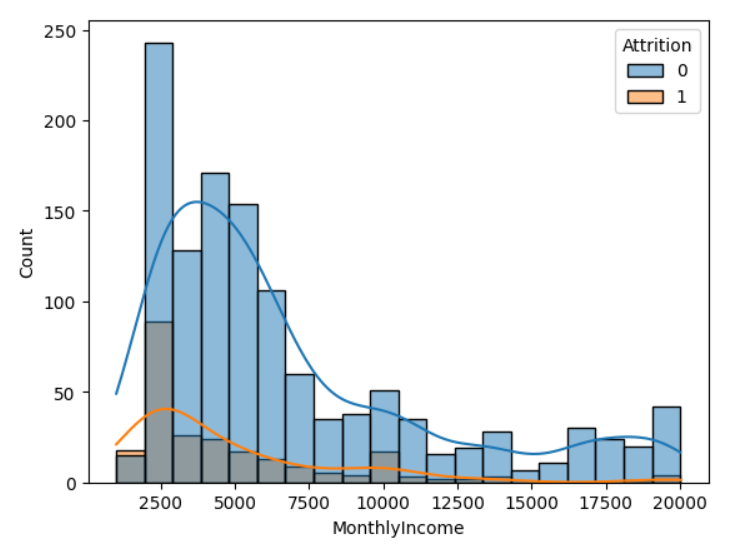
\includegraphics[width=0.7\textwidth]{monthly_income_dist.png}
\caption{Analisi della distribuzione del reddito mensile (\texttt{MonthlyIncome}) in base allo stato di \texttt{Attrition}.}
\label{fig:monthly_income_dist}
\end{figure}

    
    \item[\textbf{H3.}] \textbf{Stato Civile (\texttt{MaritalStatus}):} \textit{Il tasso di turnover è più elevato tra i dipendenti single?}
    \begin{itemize}
        \item[] I dati campionari confermano tale tendenza: i dipendenti \textit{Single} presentano un tasso di \textit{attrition} pari al \textbf{25.53\%}, un valore nettamente superiore rispetto a quello registrato per i dipendenti coniugati o divorziati, che si attesta invece all'\textbf{11.70\%}. Una possibile spiegazione sociologica e logistica risiede nel fatto che i lavoratori non legati da vincoli coniugali o familiari stabili beneficiano di una maggiore flessibilità personale, che si traduce in una più elevata disponibilità a cambiare impiego, ricollocarsi sul mercato o trasferirsi in altre città per cogliere nuove e più stimolanti opportunità professionali.
    \end{itemize}


 \item[\textbf{H4.}] \textbf{Età Anagrafica (\texttt{Age}):} \textit{Il tasso di turnover è più elevato tra le fasce anagrafiche più giovani?}
    \begin{itemize}
        \item[] I dipendenti che hanno lasciato l'azienda risultano mediamente più giovani rispetto a quelli rimasti. La distribuzione dell'età (mostrata in Figura~\ref{fig:age_dist}) evidenzia una maggiore concentrazione di casi di \textit{attrition} nelle fasce anagrafiche più basse (sotto i 40 anni, compreso), suggerendo che i lavoratori più giovani siano maggiormente propensi a cambiare impiego alla ricerca di migliori opportunità di carriera, crescita professionale o condizioni lavorative più favorevoli.
    \end{itemize}

    \begin{figure}[H]
    \centering
    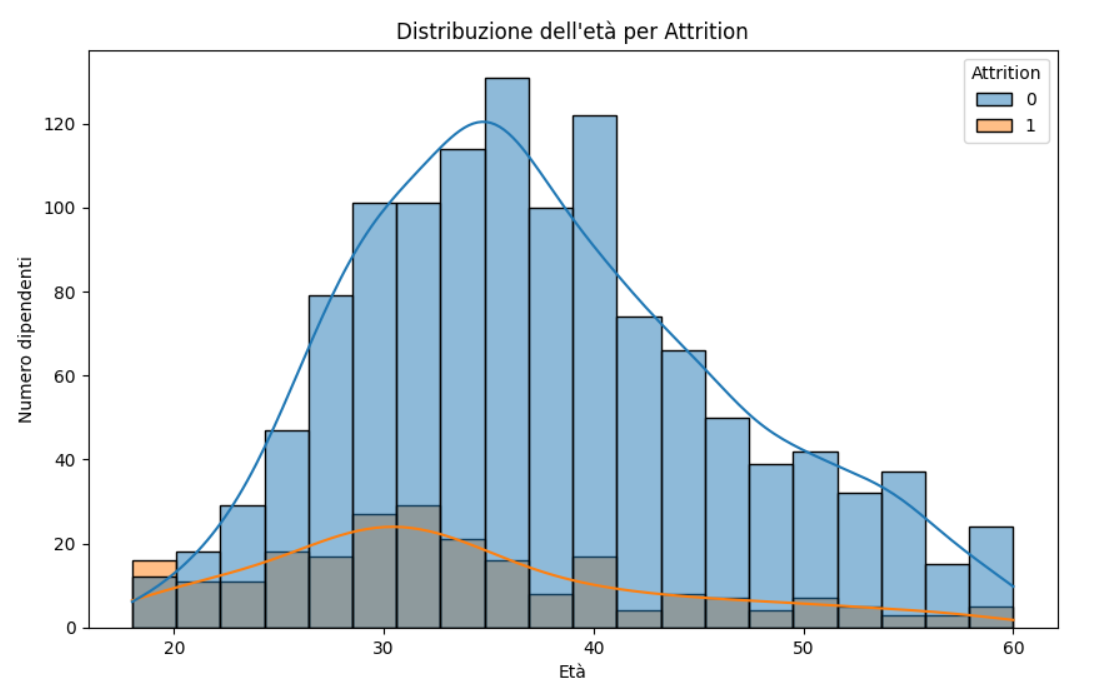
\includegraphics[width=0.7\textwidth]{age_dist.png} % Inserisci qui il nome corretto del file immagine dell'età
    \caption{Analisi della distribuzione dell'età anagrafica (\texttt{Age}) in base allo stato di \texttt{Attrition}.}
    \label{fig:age_dist}
    \end{figure}
\item[\textbf{H5.}] \textbf{Trasferte di Lavoro (\texttt{BusinessTravel}):} \textit{Il tasso di turnover è più elevato tra i dipendenti che viaggiano frequentemente per lavoro?}
    \begin{itemize}
        \item[] I riscontri empirici evidenziano che i dipendenti che viaggiano frequentemente per motivi di lavoro (\textit{Travel\_Frequently}) mostrano un tasso di \textit{attrition} nettamente superiore, pari a circa il \textbf{25\%} ($24.91\%$), rispetto alla quota riscontrata tra gli altri dipendenti che si spostano raramente o mai, la quale si attesta intorno al \textbf{14\%} ($14.08\%$). Una possibile spiegazione interpretativa risiede nel fatto che i frequenti spostamenti e la condotta di trasferte sistematiche possano incidere negativamente sull'equilibrio tra vita privata e lavoro (\textit{work-life balance}), esacerbando il rischio di insoddisfazione logistica, stress da viaggio e conseguente abbandono dell'organizzazione.
    \end{itemize}

    \item[\textbf{H6.}] \textbf{Soddisfazione Lavorativa (\texttt{JobSatisfaction}):} \textit{Una bassa soddisfazione lavorativa è correlata a un incremento del tasso di turnover?}
    \begin{itemize}
        \item[] Esiste un legame diretto tra la percezione soggettiva del proprio ruolo e la fidelizzazione; livelli bassi di soddisfazione sul lavoro risultano fortemente correlati a fenomeni di abbandono volontario. L'analisi evidenzia una relazione inversa tra soddisfazione lavorativa e \textit{attrition} (come illustrato in Figura~\ref{fig:job_satisfaction_dist}). I dipendenti con livelli più bassi di \texttt{JobSatisfaction} mostrano una maggiore probabilità di lasciare l'azienda, mentre coloro che dichiarano livelli elevati di soddisfazione tendono a rimanere più a lungo. Questo suggerisce che la soddisfazione lavorativa rappresenti un fattore rilevante nella \textit{retention} del personale.
    \end{itemize}

    \begin{figure}[H]
    \centering
    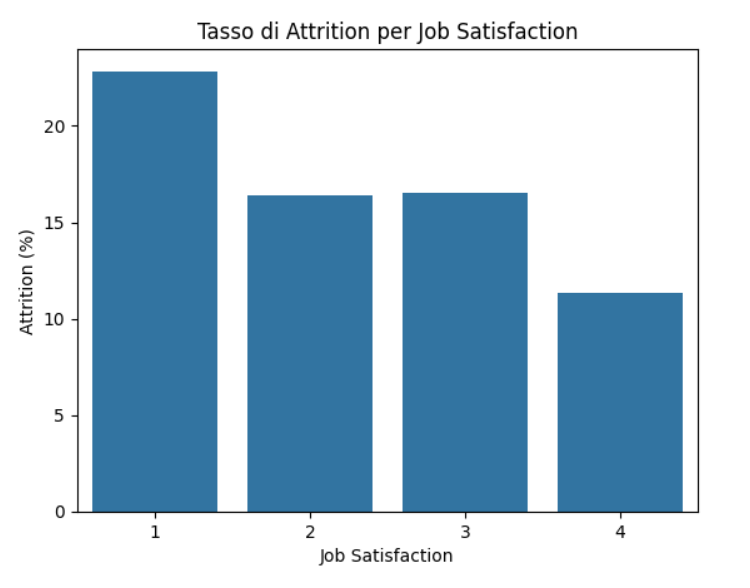
\includegraphics[width=0.7\textwidth]{job_satisfaction_dist.png} 
    \caption{Tasso di \texttt{Attrition} (\%) in base ai livelli di Soddisfazione Lavorativa (\texttt{JobSatisfaction}).}
    \label{fig:job_satisfaction_dist}
    \end{figure}

   \item[\textbf{H7.}] \textbf{Valutazione delle Prestazioni (\texttt{PerformanceRating}):} \textit{Il tasso di turnover varia in base alla valutazione delle prestazioni dei dipendenti?}
    \begin{itemize}
        \item[] I tassi di \textit{attrition} calcolati mostrano valori quasi identici tra le classi, attestandosi al \textbf{16.08\%} per i dipendenti con valutazione pari a 3 e al \textbf{16.37\%} per quelli con valutazione pari a 4. La variabile \texttt{PerformanceRating} presenta infatti una bassissima variabilità, essendo concentrata quasi esclusivamente nei soli valori 3 e 4. Questa caratteristica strutturale potrebbe fortemente limitarne il potere esplicativo e la sua reale utilità nella modellazione predittiva dell'ottimizzazione del \textit{turnover}, non delineando quei comportamenti differenti attesi tra profili a bassa produttività e \textit{top performer}.
    \end{itemize}


\item[\textbf{H8.}] \textbf{Livello di Stock Option (\texttt{StockOptionLevel}):} \textit{I dipendenti con un pacchetto azionario (Stock Option Level) più alto mostrano una maggiore propensione a rimanere in azienda?}
    \begin{itemize}
        \item[] L'assegnazione di incentivi azionari funge da efficace strumento di \textit{retention}, tuttavia l'ipotesi formulata risulta solo parzialmente confermata dai dati. L'analisi mostra che i dipendenti privi di incentivi azionari (\texttt{StockOptionLevel} = 0) presentano il più alto tasso di \textit{attrition} (\textbf{24.41\%}). I livelli 1 (\textbf{9.40\%}) e 2 (\textbf{7.59\%}) sono associati a una significativa riduzione dell'abbandono, suggerendo che la presenza di pacchetti azionari favorisca effettivamente la permanenza in azienda. Tuttavia, il livello massimo 3 non segue la medesima tendenza e registra un incremento del tasso di \textit{attrition}, pari al \textbf{17.65\%}. 
        
        La relazione tra \texttt{StockOptionLevel} e \texttt{Attrition} non è quindi monotona: sebbene i lavoratori non monetizzati mostrino il picco di abbandono, il livello più elevato di benefit (3) non corrisponde affatto al tasso di sfoltimento minimo. Ciò suggerisce la possibile covarianza di altri fattori concomitanti (come l'anzianità di ruolo o la seniority) che influenzano simultaneamente la stabilità e la permanenza del personale all'interno dell'organizzazione.
    \end{itemize}
\end{enumerate}

\section{Analisi Esplorativa dei Dati (EDA)}
L'analisi esplorativa dei dati (EDA) si pone l'obiettivo di esaminare le interazioni chiave tra le caratteristiche dei dipendenti e la variabile target \texttt{Attrition}. Per orientare l'indagine in modo quantitativo, è stata inizialmente calcolata la matrice di correlazione lineare (espressa tramite il coefficiente di Pearson) tra ciascun predittore e l'abbandono aziendale. 

I coefficienti estratti evidenziano che la variabile maggiormente associata in senso positivo all'\textit{attrition} è lo svolgimento di ore straordinarie (\texttt{OverTime\_yes} = $0.246$), seguita dallo stato civile di chi è celibe o nubile (\texttt{MaritalStatus\_single} = $0.175$) e dal ruolo specifico di rappresentante commerciale (\texttt{JobRole\_sales representative} = $0.157$). Sebbene le correlazioni si attestino su livelli moderati, esse suggeriscono preliminarmente che il carico di lavoro pressante, la situazione macro-personale e la tipologia di mansione svolta configurino fattori di rischio rilevanti nel favorire l'uscita dall'organizzazione.

Sul fronte opposto, le correlazioni negative più marcate indicano una relazione di proporzionalità inversa con la fidelizzazione: i dipendenti caratterizzati da una maggiore anzianità lavorativa complessiva (\texttt{TotalWorkingYears}  $-0.171$), livelli gerarchici più elevati (\texttt{JobLevel}  $-0.169$), stabilità nel ruolo attuale (\texttt{YearsInCurrentRole}  $-0.161$) e redditi mensili più alti (\texttt{MonthlyIncome}  $-0.159$) manifestano una propensione all'abbandono decisamente inferiore. Infine, si riscontra come la valutazione delle prestazioni (\texttt{PerformanceRating} = $0.003$) presenti una correlazione praticamente nulla con il target, suggerendo l'indipendenza statistica di tale fattore rispetto alle dinamiche di \textit{turnover} all'interno del dataset esaminato.

Al fine di approfondire queste evidenze e validare le ipotesi di ricerca in contesti multivariati, vengono strutturate e condotte le seguenti sei analisi dettagliate: Analisi per ruolo Professionale (\texttt{JobRole}), Interazione tra stato civile e straordinari (\texttt{MaritalStatus} e \texttt{OverTime}), Bilanciamento vita-lavoro e reddito (\texttt{WorkLifeBalance} e \texttt{MonthlyIncome}), Dinamica età -  reddito (\texttt{Age} e \texttt{MonthlyIncome}), Anzianità aziendale e mancata promozione (\texttt{YearsAtCompany} e \texttt{YearsSinceLastPromotion}) e infine modellazione del Risk Score. 

\subsection{Analisi per Ruolo Professionale (\texttt{JobRole})}
\textit{Quali Job Role hanno il tasso di abbandono più alto?}

Per rispondere a questo interrogativo, è stato calcolato e confrontato il tasso percentuale di \textit{attrition} all'interno di ciascuna mansione aziendale. I risultati di questa scomposizione sono riportati in Figura~\ref{fig:attrition_job_role}.

\begin{figure}[H]
\centering
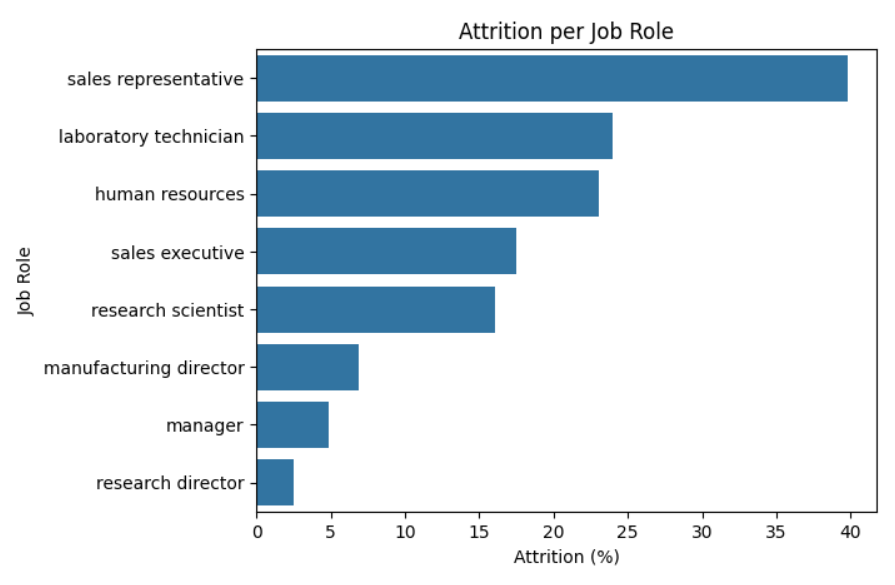
\includegraphics[width=0.85\textwidth]{image_8c9b82.png}
\caption{Tasso di \texttt{Attrition} (\%) stratificato per ruolo professionale (\texttt{JobRole}).}
\label{fig:attrition_job_role}
\end{figure}

L'analisi del tasso di abbandono per ruolo evidenzia differenze importanti tra le mansioni. I ruoli più operativi e commerciali mostrano una maggiore probabilità di abbandono rispetto alle posizioni manageriali e direttive. In particolare, i \textit{Sales Representative} (che registrano il picco massimo sfiorando il \textbf{40\%} di sfoltimento) e i \textit{Laboratory Technician} (attorno al \textbf{24\%}) risultano tra i ruoli più esposti all'\textit{attrition}. 

Al contrario, i ruoli senior come \textit{Manager} (circa \textbf{5\%}) e \textit{Research Director} (con una quota minima prossima al \textbf{2.5\%}) mostrano maggiore stabilità. Questo divario suggerisce che le mansioni caratterizzate da un'alta pressione commerciale, compiti ripetitivi o minori prospettive di crescita immediata risentano di dinamiche di ricambio molto più accentuate rispetto alle cariche apicali e di coordinamento.

\subsection{Interazione tra Stato Civile e Straordinari (\texttt{MaritalStatus} e \texttt{OverTime})}
\textit{Fare straordinari e lo stato civile che influenza hanno sulla Attrition?}

Al fine di rispondere alla domanda, viene proposto un confronto visivo diretto dei tassi di abbandono in Figura~\ref{fig:overtime_marital_attrition}.

\begin{figure}[H]
\centering
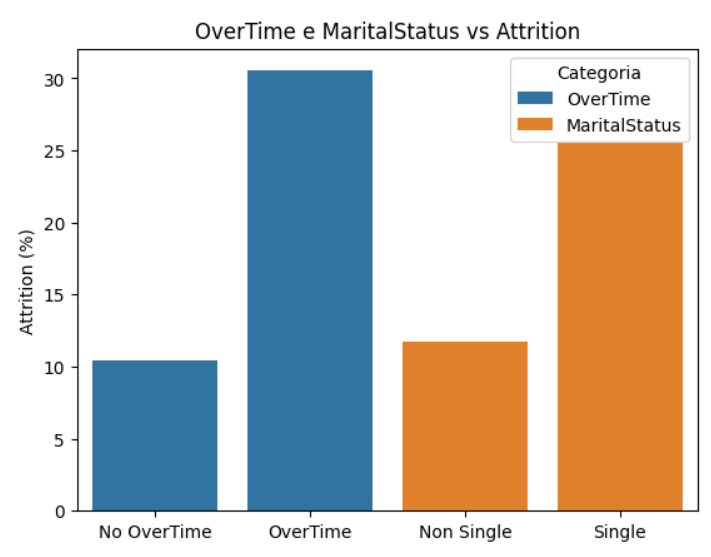
\includegraphics[width=0.85\textwidth]{image_8ca6a1.png}
\caption{Confronto del tasso di \texttt{Attrition} (\%) tra le categorie di lavoro straordinario (\texttt{OverTime}) e stato civile (\texttt{MaritalStatus}).}
\label{fig:overtime_marital_attrition}
\end{figure}

Il confronto mostra che sia lo svolgimento di straordinari sia lo stato civile single sono associati a un aumento del tasso di abbandono. I risultati sono coerenti con l'analisi delle correlazioni: \texttt{OverTime} è la variabile con la correlazione positiva più alta con \texttt{Attrition} ($r \approx 0.25$), registrando una quota di sfoltimento superiore al \textbf{30\%}, mentre \texttt{MaritalStatus\_single} mostra una correlazione positiva più moderata ($r \approx 0.18$), con un tasso di abbandono che supera il \textbf{25\%}. 

Questi dati confermano l'ipotesi che l'interazione tra l'assenza di vincoli familiari stabili (stato civile single) e l'esposizione a ritmi di lavoro pressanti (straordinari) agisca da forte catalizzatore nell'incrementare la vulnerabilità del dipendente al fenomeno del \textit{turnover} volontario.


\subsection{Bilanciamento Vita-Lavoro e Reddito (\texttt{WorkLifeBalance} e \texttt{MonthlyIncome})}
\textit{Il reddito mensile cambia in base al WorkLifeBalance e all'Attrition?}

Per investigare se esista un effetto di compensazione interattivo tra la stabilità economica e la qualità del tempo privato, viene esaminata la distribuzione congiunta tramite il grafico a violino riportato in Figura~\ref{fig:violin_wlb_income}.

\begin{figure}[H]
\centering
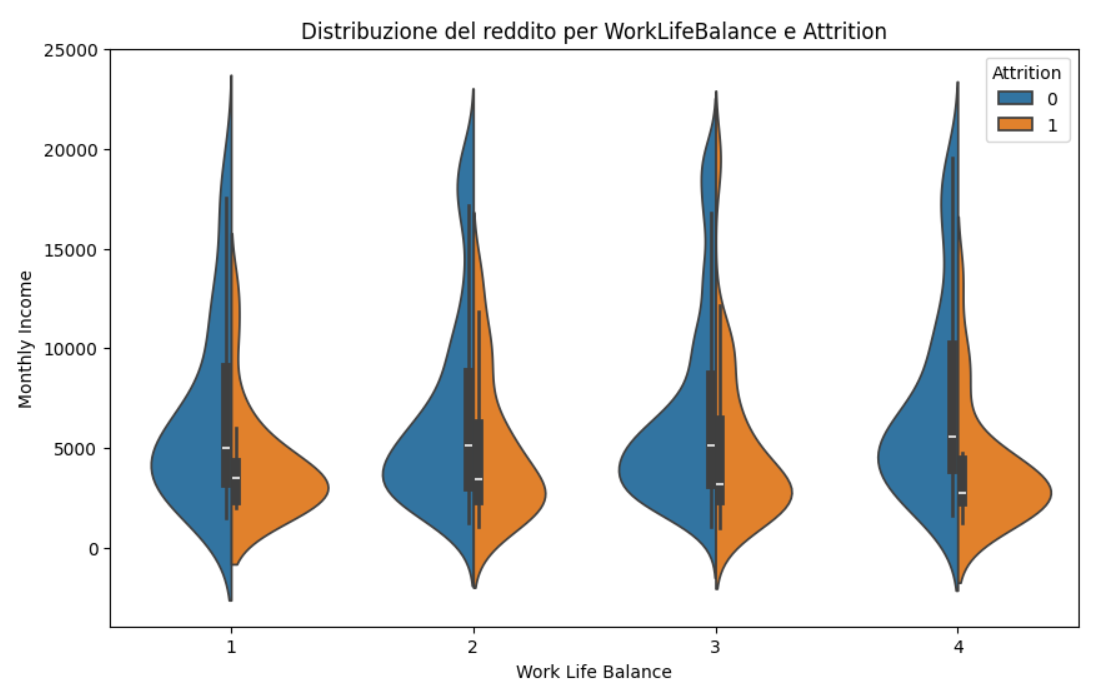
\includegraphics[width=0.9\textwidth]{image_8d1b00.png}
\caption{Distribuzione del reddito mensile (\texttt{MonthlyIncome}) per livello di \texttt{WorkLifeBalance} e stato di \texttt{Attrition}.}
\label{fig:violin_wlb_income}
\end{figure}

Il violin plot mostra la distribuzione del reddito mensile in relazione al livello di \texttt{WorkLifeBalance} e all'attrition. I dipendenti che abbandonano l'azienda tendono a concentrarsi su livelli di reddito inferiori rispetto a chi rimane, indipendentemente dal livello di equilibrio vita-lavoro. Questo suggerisce che il reddito rappresenti un fattore altamente rilevante nella permanenza aziendale.

Osservando più nel dettaglio la morfologia delle distribuzioni in Figura~\ref{fig:violin_wlb_income}:
\begin{itemize}
    \item \textbf{Asimmetria e Mediane:} Per tutte e quattro le classi di \texttt{WorkLifeBalance}, la sezione destra di ciascun violino (corrispondente ad \texttt{Attrition} = 1, in arancione) mostra una vistosa pancia concentrata nella fascia a basso reddito (tra i \$2.500 e i \$5.000) e linee mediane strutturalmente più basse rispetto alla controparte che rimane in azienda (\texttt{Attrition} = 0, in blu).
    \item \textbf{Assenza di Effetto Compensativo:} Anche nei cluster caratterizzati da un ottimo bilanciamento della vita privata (\texttt{WorkLifeBalance} = 3 ed \texttt{WorkLifeBalance} = 4), i dipendenti con retribuzioni modeste continuano a mostrare tassi significativi di abbandono. Ciò dimostra empiricamente che una buona flessibilità e un ambiente di lavoro sereno non riescono a controbilanciare o neutralizzare la spinta all'allontanamento generata da una remunerazione percepita come insufficiente.
\end{itemize}

\subsection{Dinamica Età-Reddito (\texttt{Age} e \texttt{MonthlyIncome})}
\textit{L'età del dipendente e il suo stipendio mensile influenzano l'abbandono?}

Per comprendere le dinamiche congiunte della stabilità economica e della maturità anagrafica rispetto ai fenomeni di sfoltimento, viene proposto lo scatter plot bivariato riportato in Figura~\ref{fig:scatter_age_income}.

\begin{figure}[H]
\centering
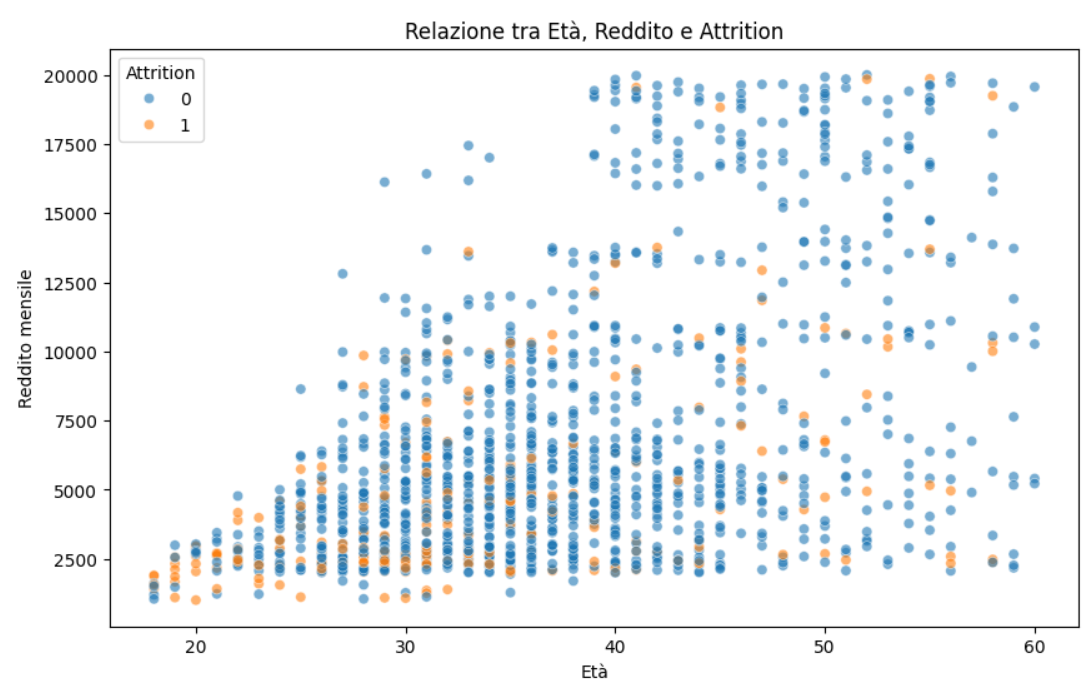
\includegraphics[width=0.9\textwidth]{image_8d2647.jpg}
\caption{Scatter plot della relazione tra Età (\texttt{Age}), Reddito Mensile (\texttt{MonthlyIncome}) e stato di \texttt{Attrition}.}
\label{fig:scatter_age_income}
\end{figure}

Lo scatterplot evidenzia una relazione tra età, reddito mensile e attrition. I casi di abbandono risultano maggiormente concentrati tra i dipendenti più giovani e con redditi inferiori, mentre i dipendenti più anziani e con maggiore reddito mostrano una maggiore stabilità. Questo suggerisce che la combinazione tra esperienza lavorativa e posizione economica possa influenzare la permanenza nell'organizzazione.

Esaminando in modo più approfondito i pattern di addensamento visibili in Figura~\ref{fig:scatter_age_income}:
\begin{itemize}
    \item \textbf{Il Cluster Critico (Giovani a basso reddito):} Si nota una forte densità di punti arancioni (\texttt{Attrition} = 1) nell'angolo in basso a sinistra del grafico, nello specifico tra i 18 e i 35 anni di età con un reddito mensile inferiore ai \$5.000. Questa fascia rappresenta il segmento aziendale a più alto rischio di mobilità uscente.
    \item \textbf{La Fascia di Stabilizzazione gerarchica:} Man mano che l'età avanza (oltre i 40 anni), il reddito mensile tende a distribuirsi su fasce più ampie (fino al tetto dei \$20.000), e la presenza di casi di sfoltimento si dirada sensibilmente. I rari punti arancioni visibili tra i dipendenti senior rimangono comunque per lo più confinati nelle fasce retributive medio-basse per quell'età, confermando che l'insoddisfazione economica agisce da trigger anche in contesti anagrafici più maturi.
\end{itemize}

\subsection{Anzianità Aziendale e Mancata Promozione}
\textit{I dipendenti che rimangono molti anni senza essere promossi hanno più probabilità di lasciare?}

Per analizzare quantitativamente l'effetto della stagnazione professionale, viene studiata la metrica normalizzata \texttt{PromotionDelayRatio} (calcolata come rapporto tra gli anni trascorsi dall'ultima promozione e gli anni totali spesi all'interno dell'azienda). La scomposizione di questo indice rispetto allo stato di fidelizzazione è illustrata tramite i boxplot intagliati in Figura~\ref{fig:boxplot_promotion_delay}.

\begin{figure}[H]
\centering
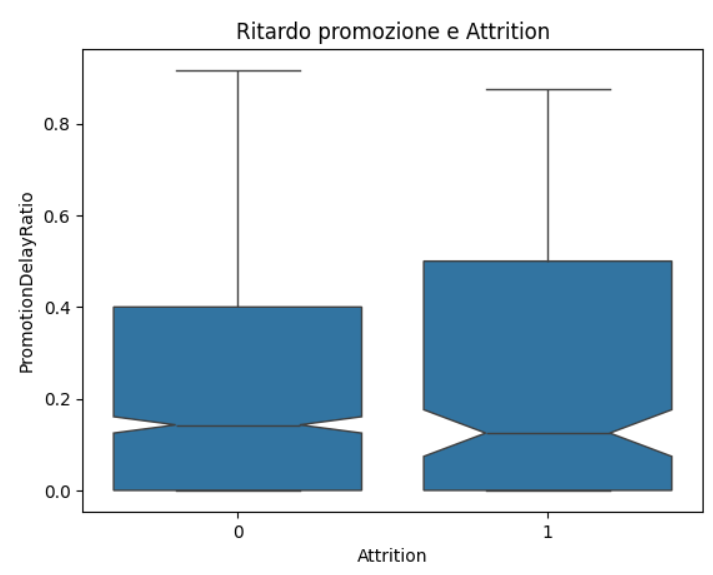
\includegraphics[width=0.75\textwidth]{image_8d2648.jpg}
\caption{Boxplot comparativo del tasso di ritardo della promozione (\texttt{PromotionDelayRatio}) in base allo stato di \texttt{Attrition}.}
\label{fig:boxplot_promotion_delay}
\end{figure}

I dipendenti che hanno trascorso una quota maggiore della propria permanenza aziendale senza una promozione mostrano una maggiore probabilità di abbandono. Questo può indicare un effetto della percezione di limitate opportunità di carriera.

Analizzando in modo più specifico la geometria dei boxplot in Figura~\ref{fig:boxplot_promotion_delay}:
\begin{itemize}
    \item \textbf{Estensione del Terzo Quartile (Q3):} Nel cluster dei dipendenti che hanno abbandonato l'organizzazione (\texttt{Attrition} = 1), la scatola si estende significativamente verso l'alto, posizionando il terzo quartile alla quota di $0.50$. Questo significa che ben il \textbf{25\%} dei lavoratori fuoriusciti ha vissuto una condizione di stasi in cui almeno la metà (o più) dell'intera carriera interna è trascorsa senza ricevere alcun avanzamento di livello o di qualifica.
    \item \textbf{Analisi degli Intagli:} Le tacche a forma di imbuto in corrispondenza delle due mediane si sovrappongono parzialmente lungo l'asse delle ordinate. Sebbene la tendenza centrale indichi che un ritardo relativo elevato esasperi il rischio di sfoltimento, la sovrapposizione geometrica dei due intervalli di confidenza suggerisce che la mancata promozione agisca raramente come fattore isolato; essa tende piuttosto a combinarsi sinergicamente con altre determinanti (come il livello salariale o il ruolo ricoperto) nel far maturare la decisione definitiva di interruzione del rapporto lavorativo.
\end{itemize}

\subsection{Modellazione del Risk Score (\texttt{RiskScore})}
\textit{Possiamo individuare un profilo di dipendente ad alto rischio?}

A conclusione dell'indagine esplorativa, l'effetto combinato delle principali determinanti emerse come critiche (lavoro straordinario, bassi livelli di reddito, stato civile single, giovane età e stagnazione di carriera) è stato sintetizzato con il nome della variabile \texttt{RiskScore}. La distribuzione del tasso di sfoltimento in base al numero di fattori di rischio simultaneamente presenti è illustrata in Figura~\ref{fig:risk_score_attrition}.

\begin{figure}[H]
\centering
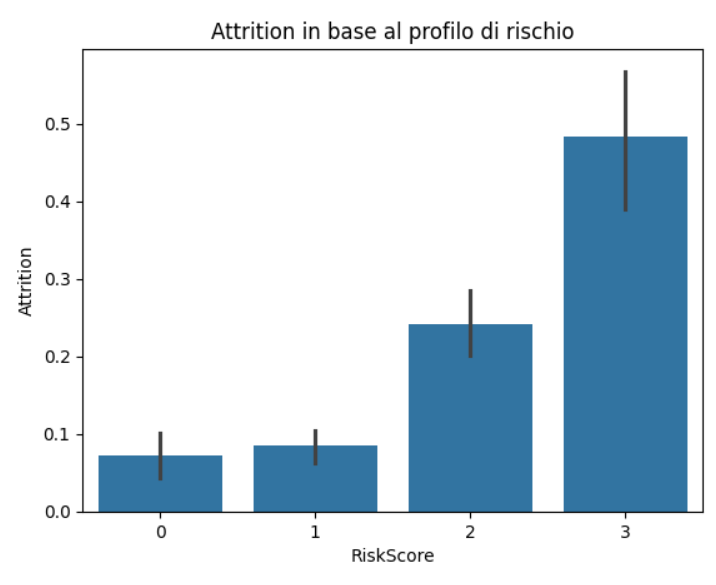
\includegraphics[width=0.75\textwidth]{image_8da2e1.png}
\caption{Tasso medio di \texttt{Attrition} in base al livello cumulativo di rischio (\texttt{RiskScore}).}
\label{fig:risk_score_attrition}
\end{figure}

L'attrition aumenta all'aumentare dei fattori di rischio combinati, suggerendo che il fenomeno dipenda dall'interazione di più condizioni. 

Esaminando in modo specifico l'andamento delle frequenze in Figura~\ref{fig:risk_score_attrition}, si possono trarre le seguenti considerazioni analitiche:
\begin{itemize}
    \item \textbf{Crescita Non Lineare:} Mentre i dipendenti caratterizzati da zero o un solo fattore di vulnerabilità mostrano una spiccata stabilità, con tassi di abbandono confinati al di sotto del \textbf{10\%}, la quota di \textit{attrition} subisce un'impennata drammatica al manifestarsi simultaneo di più criticità. Per un \texttt{RiskScore} pari a 2, la percentuale sale oltre il \textbf{20\%} ($24\%$), per poi sfiorare la soglia critica del \textbf{50\%} ($48\%$) in corrispondenza del livello di rischio 3.
    \item \textbf{Intervalli di Confidenza:} Le linee verticali nere poste sulla sommità di ciascuna barra rappresentano la variabilità campionaria della stima. L'estensione maggiore visibile sul livello 3 indica che, sebbene la tendenza all'allontanamento sia nettamente prevalente in questo cluster, la numerosità campionaria ridotta di dipendenti che accumulano contemporaneamente così tante penalizzazioni introduce una variabilità superiore, che merita un monitoraggio analitico isolato in fase di modellazione predittiva.
\end{itemize}

\section{Modellazione}
Una volta conclusa la fase di analisi esplorativa e compresi i principali driver legati all'allontanamento volontario del personale, l'obiettivo si sposta sulla costruzione di una funzione predittiva in grado di mappare le caratteristiche dei dipendenti verso la variabile target binaria \texttt{Attrition}. Per rispondere in modo robusto a questa sfida di classificazione, la pipeline computazionale prevede l'addestramento e l'ottimizzazione di tre diversi algoritmi di Machine Learning, caratterizzati da complessità e assunzioni matematiche differenti:
\begin{itemize}
    \item \textbf{Regressione Logistica} 
    \item \textbf{K-Nearest Neighbors ($K$-NN)} 
    \item \textbf{Random Forest} 
\end{itemize}

\subsection{Regressione Logistica}

Il primo modello è la Regressione Logistica, un algoritmo di apprendimento utilizzato per problemi di classificazione. A differenza della regressione lineare, che ha come obiettivo la previsione di variabili continue, la regressione logistica modella la probabilità che una determinata osservazione appartenga a una specifica classe.

In particolare, questo metodo è impiegato per problemi di classificazione binaria, in cui l’output può assumere due possibili valori, come ad esempio Yes/No, True/False oppure 0/1 \cite{gfg-logistic}.

Dal punto di vista matematico, il modello utilizza la funzione sigmoide per trasformare la combinazione lineare delle variabili esplicative in una probabilità compresa tra 0 e 1.. Lo addestriamo sui dati scalati e lo valutiamo sul test set con accuracy, matrice di confusione e classification report (precision, recall, f1-score). I risultati completi di questa valutazione sono mostrati in Figura~\ref{fig:log_reg_results}.

\begin{figure}[H]
\centering
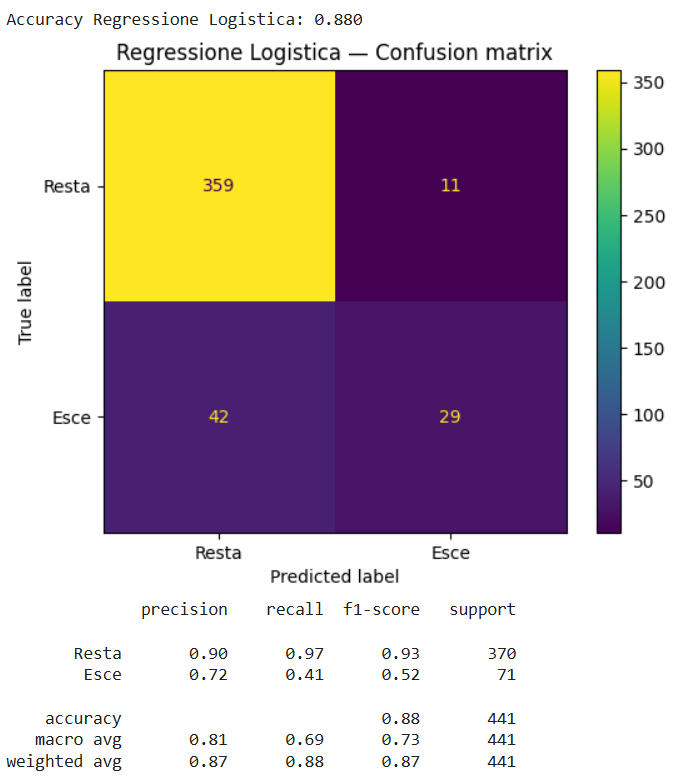
\includegraphics[width=0.75\textwidth]{image_ca3fe5.png}
\caption{Matrice di confusione e metriche di classificazione per la Regressione Logistica.}
\label{fig:log_reg_results}
\end{figure}

\subsubsection{Interpretazione Analitica}
Il modello raggiunge un'accuracy dell'88\% ($0.880$), ma questo valore va letto con cautela per via dello sbilanciamento delle classi: poiché l'84\% dei dipendenti resta, un modello banale che prevedesse "Resta" per tutti otterrebbe già circa l'84\% di accuracy. È quindi più informativo guardare le metriche sulla classe "Esce", quella di reale interesse. Qui la precision è 0.72 e il recall 0.41: il modello individua il 41\% dei dipendenti che effettivamente se ne vanno, e quando prevede "Esce" ha ragione nel 72\% dei casi. L'f1-score sulla classe "Esce" è 0.52, il più alto tra i tre modelli.

Un esame più dettagliato della matrice di confusione e del report in Figura~\ref{fig:log_reg_results} consente di trarre le seguenti considerazioni geometriche e statistiche:
\begin{itemize}
    \item \textbf{Predizione della Retention (Classe "Resta"):} Il modello dimostra un'elevata accuratezza nel riconoscere i dipendenti stabili, identificando correttamente \textbf{359} Veri Negativi (dipendenti che rimangono e sono previsti come tali) e commettendo solo \textbf{11} errori di Falso Positivo (dipendenti che rimangono ma erano stati classificati a rischio uscita). Questo si traduce in una precision del $0.90$ e in un recall del $0.97$ su un supporto di 370 istanze.
    \item \textbf{Il Limite del Modello (Falsi Negativi):} Il limite principale risiede nei \textbf{42} casi di Falso Negativo posizionati nel quadrante inferiore sinistro. Si tratta di dipendenti che hanno effettivamente interrotto il proprio rapporto di lavoro ma che il modello ha erroneamente etichettato come "Resta". Questa forte incidenza comprime il valore di recall a $0.41$ su 71 casi totali di abbandono, evidenziando come l'iperpiano di separazione lineare risenta dello sbilanciamento originario dei dati pur mantenendo una buona precisione complessiva ($0.72$) quando decide di lanciare un segnale d'allarme.
\end{itemize}

\subsection{k-Nearest Neighbors (k-NN)}

Il secondo modello è il k-Nearest Neighbors, un algoritmo di apprendimento utilizzato per problemi di classificazione e regressione. Il principio alla base del metodo consiste nell’identificare, per una data osservazione, i $k$ esempi più vicini nello spazio e nel determinare la previsione attraverso un meccanismo di aggregazione locale, come la classe maggioritaria o la media dei valori osservati \cite{gfg-knn}.



Essendo basato sulle distanze, va addestrato sui dati scalati. La valutazione completa del classificatore sul test set è riportata in Figura~\ref{fig:knn_results}.

\FloatBarrier

\begin{figure}[H]
\centering
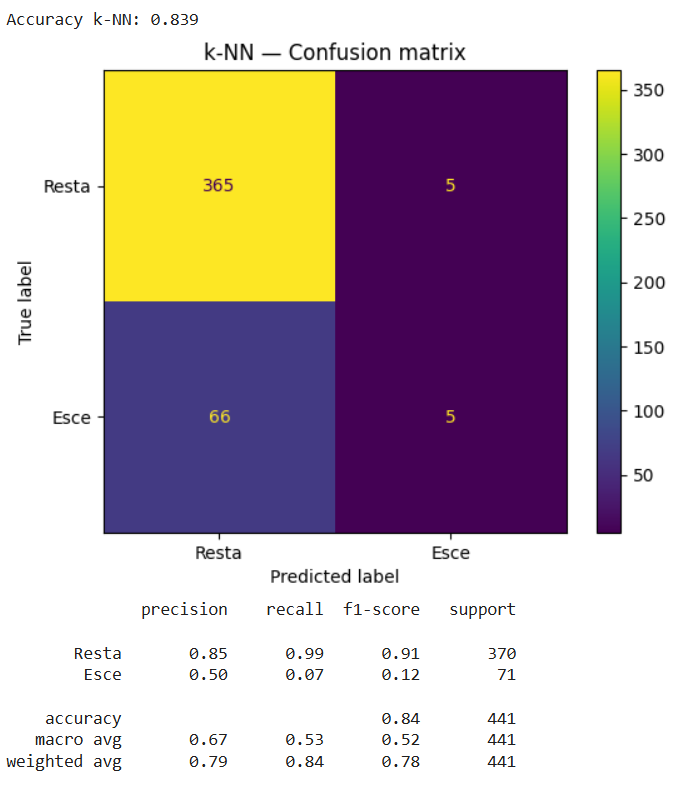
\includegraphics[width=0.65\textwidth]{image_ca5625.png}
\caption{Matrice di confusione e metriche di classificazione per il modello k-NN.}
\label{fig:knn_results}
\end{figure}

\subsubsection{Interpretazione Analitica}
Pur avendo un'accuracy dell'84\% ($0.839$), in linea con gli altri modelli, il k-NN risulta poco utile per il nostro obiettivo. Il recall sulla classe "Esce" è solo 0.07: il modello individua appena il 7\% dei dipendenti che se ne vanno, classificando quasi tutti come "Resta". Questo è un esempio chiaro di come l'accuracy possa essere fuorviante con classi sbilanciate: il modello ottiene un valore alto semplicemente assecondando la classe maggioritaria. L'f1-score sulla classe "Esce" è 0.12, il più basso tra i tre modelli.

L'analisi della matrice di confusione e del relativo classification report in Figura~\ref{fig:knn_results} mette in luce la criticità geometrica dell'algoritmo in presenza di \textit{class imbalance}:
\begin{itemize}
    \item \textbf{Schiacciamento sulla classe maggioritaria:} Il modello assegna quasi la totalità delle istanze alla classe "Resta", totalizzando ben \textbf{365} Veri Negativi e commettendo solo \textbf{5} Falsi Positivi. Questo comportamento pigro (\textit{lazy}) genera un recall fittizio del $0.99$ sulla stabilità aziendale.
    \item \textbf{Incapacità di intercettare il turnover:} A fronte di 71 dipendenti che hanno realmente abbandonato l'azienda (supporto della classe "Esce"), il $k$-NN ne individua correttamente soltanto \textbf{5} (Veri Positivi), commettendo ben \textbf{66} errori di Falso Negativo. 
\end{itemize}


\subsection{Random Forest}

Il terzo modello è il Random Forest, un algoritmo di apprendimento supervisionato basato su un approccio \textit{ensemble}, che combina un insieme di alberi decisionali per ottenere previsioni più accurate e robuste. Ciascun albero viene addestrato su un sottocampione casuale del dataset e considera, a ogni nodo, un sottoinsieme casuale delle variabili esplicative.

Le singole previsioni degli alberi vengono successivamente aggregate: nel caso di classificazione tramite voto di maggioranza, mentre nei problemi di regressione attraverso la media dei valori predetti.

Grazie a questa procedura di aggregazione, la Random Forest è in grado di ridurre la varianza dei singoli modelli e migliorare le prestazioni predictive complessive, limitando al contempo il rischio di overfitting rispetto ai singoli alberi decisionali \cite{gfg-randomforest}.

Lo addestriamo sui dati non scalati. Usiamo \texttt{n\_estimators=200} e \texttt{random\_state=42} per la riproducibilità. La valutazione delle prestazioni sul test set è illustrata in Figura~\ref{fig:random_forest_results}.

\begin{figure}[H]
\centering
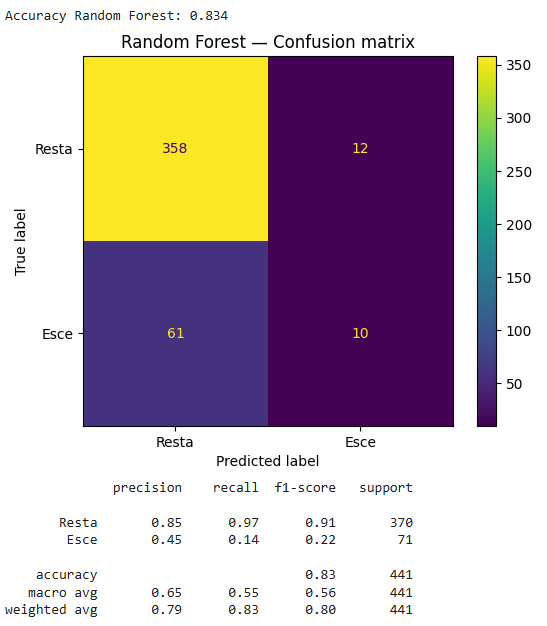
\includegraphics[width=0.70\textwidth]{image_cb21f3.png}
\caption{Matrice di confusione e metriche di classificazione per il modello Random Forest.}
\label{fig:random_forest_results}
\end{figure}

\subsubsection{Interpretazione Analitica}
La Random Forest ottiene un'accuracy dell'83\% ($0.834$), ma anche in questo caso le prestazioni sulla classe "Esce" sono limitate: recall 0.14 e precision 0.45, per un f1-score di 0.22. Il modello individua quindi solo il 14\% di chi se ne va. Pur essendo più sofisticato del k-NN, non riesce a gestire bene lo sbilanciamento e resta nettamente inferiore alla Regressione Logistica su questo problema.

L'ispezione della matrice di confusione e del report delle metriche in Figura~\ref{fig:random_forest_results} evidenzia i seguenti aspetti:
\begin{itemize}
    \item \textbf{Gestione della classe maggioritaria:} Il modello individua correttamente \textbf{358} Veri Negativi (dipendenti che rimangono), commettendo \textbf{12} errori di Falso Positivo, dimostrando un comportamento solido ma sbilanciato sul campione dominante, in modo analogo a quanto osservato per i classificatori precedenti.
    \item \textbf{Difficoltà con il turn-over:} A fronte delle 71 cessazioni effettive nel test set, la Random Forest cattura come Veri Positivi soltanto \textbf{10} istanze, lasciando ben \textbf{61} Falsi Negativi non rilevati. Nonostante l'architettura a macro-insieme (\textit{ensemble}) schieri 200 alberi decisionali indipendenti, la prevalenza statistica dei record di fidelizzazione condiziona la selezione delle soglie di split nei nodi, limitando drasticamente la sensibilità del modello verso la classe minoritaria.
\end{itemize}



\subsection{Confronto Comparativo tra i Modelli}

Per confrontare i tre modelli li mettiamo a confronto sulle metriche principali. Oltre all'accuracy complessiva riportiamo precision, recall e f1-score sulla classe "Esce", che è quella di reale interesse e su cui lo sbilanciamento incide di più. I risultati sono raccolti all'interno della Tabella~\ref{tab:confronto_modelli}.

\begin{table}[H]
\centering
\caption{Quadro comparativo delle performance dei modelli sulla classe minoritaria (\texttt{Attrition} = 1).}
\label{tab:confronto_modelli}
\begin{tabularx}{\textwidth}{Xcccc}
\toprule
\textbf{Modello} & \textbf{Accuracy} & \textbf{Precision (Esce)} & \textbf{Recall (Esce)} & \textbf{F1-Score (Esce)} \\ 
\midrule
Regressione Logistica & 0.880 & 0.725 & 0.408 & 0.523 \\ 
k-NN                  & 0.839 & 0.500 & 0.070 & 0.123 \\ 
Random Forest         & 0.834 & 0.455 & 0.141 & 0.215 \\ 
\bottomrule
\end{tabularx}
\end{table}

\subsubsection{Interpretazione del Confronto}
I tre modelli hanno un'accuracy simile (0.83–0.88), ma questo valore è poco informativo a causa dello sbilanciamento delle classi. Il confronto più significativo è sull'f1-score della classe "Esce": la Regressione Logistica (0.52) supera nettamente Random Forest (0.22) e k-NN (0.12). La Regressione Logistica è quindi il modello migliore per questo problema, sia per capacità di individuare i dipendenti a rischio (recall 0.41, il più alto) sia per affidabilità delle sue previsioni positive (precision 0.72, la più alta). È un risultato interessante perché il modello più semplice e interpretabile risulta anche il più efficace, a conferma che la complessità di un modello non garantisce prestazioni migliori.

Analizzando in maniera approfondita i dati espressi nella Tabella~\ref{tab:confronto_modelli}, emergono considerazioni fondamentali relative alla natura geometrica dei classificatori in contesti fortemente asimmetrici:
\begin{itemize}
    \item \textbf{Il fallimento degli approcci locali e non lineari:} Il modello $k$-NN, basandosi su metriche di distanza pura, soffre drammaticamente l'addensamento spaziale della classe maggioritaria, crollando a un recall critico del $0.070$. Anche l'architettura Random Forest, pur sfruttando la non-linearità degli insiemi di alberi, risente di un marcato condizionamento nelle foglie, fermando il proprio recupero a un modesto $0.141$.
    \item \textbf{La superiorità del confine lineare:} La Regressione Logistica riesce a strutturare un iperpiano separatore più efficace, massimizzando contemporaneamente l'affidabilità quando assegna il target positivo (precision pari a $0.725$) e catturando oltre il \textbf{40\%} dei reali casi di abbandono aziendale.
\end{itemize}


\section{Risultati e Discussione}
L’analisi quantitativa e l’indagine esplorativa condotte sul dataset hanno permesso di mappare analiticamente i fattori chiave che governano il fenomeno dell’\textit{employee attrition}. I riscontri ottenuti confermano che l’abbandono dei dipendenti non risponde a una singola determinante isolata, ma si configura come il risultato combinato dell'interazione sinergica tra più dimensioni economiche, professionali, psicometriche e personali.

Al fine di fornire un quadro d'insieme rigoroso, la Tabella~\ref{tab:sintesi_ipotesi} riassume lo stato di validazione delle ipotesi di ricerca precedentemente formalizzate nella Sezione 2.

\begin{table}[H]
\centering
\caption{Matrice di sintesi e validazione delle ipotesi di ricerca.}
\label{tab:sintesi_ipotesi}

\begin{tabularx}{\textwidth}{l l X l}
\hline
\textbf{Cod.} & \textbf{Predittore Esaminato} & \textbf{Effetto su Attrition} & \textbf{Esito Ipotesi} \\ 
\hline
\textbf{H1} & Lavoro Straordinario (\texttt{OverTime}) & Incremento lineare marcato & \textbf{Confermata} \\
\textbf{H2} & Reddito Mensile (\texttt{MonthlyIncome}) & Forte concentrazione nelle fasce basse & \textbf{Confermata} \\
\textbf{H3} & Stato Civile (\texttt{MaritalStatus}) & Picco nel cluster \textit{Single} & \textbf{Confermata} \\
\textbf{H4} & Età Anagrafica (\texttt{Age}) & Maggiore incidenza under 40 & \textbf{Confermata} \\
\textbf{H5} & Trasferte di Lavoro (\texttt{BusinessTravel}) & Incremento per \textit{Travel\_Frequently} & \textbf{Confermata} \\
\textbf{H6} & Soddisfazione (\texttt{JobSatisfaction}) & Relazione inversa sulle classi Likert & \textbf{Confermata} \\
\textbf{H7} & Valutazione (\texttt{PerformanceRating}) & Nessuna variabilità statistica ($r \approx 0$) & \textbf{Rifiutata} \\
\textbf{H8} & Benefit (\texttt{StockOptionLevel}) & Relazione non monotona (U-shaped) & \textbf{Parz. Confermata} \\
\hline
\end{tabularx}
\end{table}

\subsection{Analisi dei driver principali e delle interazioni}
Emerge con assoluta forza il ruolo del \textbf{lavoro straordinario (\texttt{OverTime})} come principale catalizzatore del rischio: i dipendenti sottoposti a regimi di lavoro intensi mostrano un'impennata del tasso di sfoltimento ($\approx 31\%$), convalidando l'ipotesi secondo cui il sovraccarico e l'usura professionale erodono la \textit{retention} aziendale.

Un secondo elemento strutturale è rappresentato dal \textbf{reddito mensile (\texttt{MonthlyIncome})}. Le distribuzioni evidenziano che i dipendenti fuoriusciti si concentrano in modo quasi esclusivo nelle fasce retributive inferiori (sotto i \$5.000). Come dimostrato dall'analisi bivariata condotta tramite violin plot, la leva economica gioca un ruolo così fondamentale da non poter essere mitigata: nemmeno un ottimo bilanciamento della vita privata (\texttt{WorkLifeBalance} elevato) è in grado di compensare o neutralizzare l'effetto di sfoltimento indotto da un salario percepito come inadeguato.

L’analisi ha inoltre evidenziato l'importanza dei fattori socio-demografici ed esistenziali. I dipendenti \textbf{single} presentano una propensione all’abbandono sensibilmente superiore rispetto ai colleghi coniugati o divorziati ($25.53\%$ contro $11.70\%$). Dal punto di vista anagrafico, tale vulnerabilità si esaspera nei \textbf{dipendenti più giovani} (under 35), i quali si trovano nella fase embrionale della carriera e risentono contemporaneamente di bassi livelli salariali d'ingresso. Al contrario, l'avanzamento dell'età anagrafica e della \textit{seniority} si associa a una progressiva stabilizzazione del rapporto di lavoro.

Sul piano organizzativo, una \textbf{bassa soddisfazione lavorativa (\texttt{JobSatisfaction})} e la frequenza strutturale di \textbf{trasferte di lavoro (\texttt{BusinessTravel})} agiscono come acceleratori del ricambio volontario. Per quanto riguarda gli incentivi di lungo periodo, il \textbf{livello di stock option} si comporta come un efficace strumento di fidelizzazione solo fino al livello 2; al livello massimo (3) si osserva un'inversione di tendenza con un aumento dell'attrition al $17.65\%$, suggerendo che un ricorso estremo ai benefit azionari si associ a profili specialistici o manageriali comunque altamente appetibili sul mercato o sottoposti a dinamiche di stress differenti. 

Infine, la \textbf{stagnazione di carriera} (misurata tramite il \texttt{PromotionDelayRatio}) ha confermato che trascorrere una quota rilevante della propria storia aziendale senza promozioni genera un senso di frustrazione che incentiva l'uscita, sebbene tale fattore esprima la sua massima forza distruttiva quando opera in concomitanza con ruoli operativi e commerciali (come i \textit{Sales Representative}).

Nel complesso, l’\textit{attrition} si dimostra un fenomeno ampiamente multidimensionale. Il calcolo del \textit{Risk Score} ha fornito la prova empirica definitiva: il rischio cresce in modo non lineare. Accumulare tre o più penalizzazioni simultanee (es. essere giovani, single e costretti agli straordinari) fa precipitare la probabilità di permanenza in azienda, portando il tasso di sfoltimento a sfiorare il \textbf{50\%}.

\subsection{Implicazioni manageriali e strategiche}
I risultati emersi offrono precisi spunti di intervento per la direzione delle Risorse Umane (\textit{HR Management}) volti a ottimizzare le politiche di \textit{retention} e salvaguardare il capitale umano aziendale:
\begin{enumerate}
    \item \textbf{Monitoraggio dei Regimi di OverTime:} Risulta prioritario implementare sistemi di auditing interno per evitare che il lavoro straordinario diventi una pratica sistematica. Qualora le ore extra siano strutturali, l'azienda deve prevedere piani di recupero obbligatori o forme di welfare compensativo per preservare il \textit{work-life balance}.
    \item \textbf{Politiche Retributive per i Profili Junior:} Poiché il cluster dei giovani a basso reddito rappresenta il segmento a più alto rischio, è fondamentale rivedere i minimi salariali d'ingresso e definire percorsi di \textit{Career Pathing} chiari e trasparenti fin dai primi mesi dall'assunzione, spezzando la combinazione stagnazione-basso reddito.
    \item \textbf{Interventi Mirati sui Ruoli Critici:} I comparti operativi e commerciali (in primis i \textit{Sales Representative}) necessitano di una completa ridefinizione dei sistemi di incentivazione e di supporto psicologico, riducendo la pressione bivariata generata dagli obiettivi di vendita e dai frequenti viaggi di lavoro.
\end{enumerate}

\section{Conclusioni}

Il presente studio ha permesso di analizzare in modo rigoroso e quantitativo le dinamiche sottostanti il fenomeno dell’\textit{employee attrition} all’interno dell’organizzazione. Attraverso un approccio strutturato di \textit{Data Science}, l’analisi esplorativa (EDA) ha evidenziato come l’abbandono aziendale non sia riconducibile a una singola causa isolata, ma derivi da un insieme di fattori interagenti di natura economica, professionale e personale.

Le evidenze empiriche raccolte delineano un profilo di rischio ben definito: la combinazione di elevati carichi di lavoro (straordinari frequenti), retribuzioni relativamente basse, stagnazione professionale e condizioni personali caratterizzate da elevata flessibilità (come giovani lavoratori single) risulta fortemente associata a una maggiore probabilità di abbandono. L’analisi del \texttt{RiskScore} ha inoltre confermato che il rischio di attrition cresce in modo non lineare all’aumentare del numero di fattori critici presenti simultaneamente.

Dal punto di vista applicativo, i risultati ottenuti presentano un duplice valore:
\begin{itemize}
    \item \textbf{Valore strategico per le risorse umane:} l’individuazione dei principali fattori di rischio consente al management di sviluppare politiche di retention mirate, come la revisione dei livelli retributivi per i profili junior, il monitoraggio dei carichi di lavoro e la progettazione di percorsi di crescita professionale più dinamici.
    
    \item \textbf{Valore analitico e computazionale:} l’identificazione dello sbilanciamento delle classi, della presenza di feature poco informative (come \texttt{PerformanceRating}) e delle relazioni tra variabili fornisce una base solida per la costruzione di modelli predittivi robusti ed efficaci.
\end{itemize}


\bibliographystyle{unsrt} 
\bibliography{riferimenti} 


\end{document}
